\chapter{Results and Analysis}
\label{ch:results}

\section{Functional correctness}

The final core regression contained 447 assertions and all passed (\cref{tab:coretests}). The runtime/resource suite was the largest source of semantic evidence, while editor GUI and GPU suites covered interactions and presentation. A 180-physics-frame arena smoke test retained three active runners and a live complex enemy. Editor launch logs for the active project, distribution template and clean-install project contained no real failure, script error, leak, crash or illegal memory access.

\begin{table}[htbp]
\centering
\caption{Final core automated regression.}
\label{tab:coretests}
\begin{tabular}{lrrp{0.43\textwidth}}
\toprule
Suite & Passed & Total & Principal coverage \\
\midrule
Resource and runtime & 153 & 153 & Structure, node semantics, decorators, actor calls, schemas, debug bridge and cache invalidation \\
Editor GUI & 185 & 185 & Graph editing, history, typed controls, schema tools, live blackboard and 19 display switches \\
Basic game & 13 & 13 & Three enemies, movement, damage, patrol, death/restart and runner lifecycle \\
Complex arena & 26 & 26 & Detection, pursuit, directional attack, search, retreat, recovery and new composite nodes \\
Real-GPU visual & 70 & 70 & Seventeen 1600 by 900 screenshots and visual invariants \\
\midrule
Total & 447 & 447 & All core assertions passed \\
\bottomrule
\end{tabular}
\end{table}

Additional suites were kept separate to avoid inflating the core total. The controlled human-study fixture passed 21 of 21 GPU assertions, runtime profiling and topology safety passed 511 of 511 assertions, and packaging passed 53 of 53 checks. The version 0.9.0 archive contained only the plugin directory, included an MIT licence and SHA-256 manifest, and enabled successfully in an otherwise empty Godot 4.6 project.

The complex-arena tests showed that agents were genuinely driven by tree execution rather than a parallel hard-coded controller. Entering detection range set blackboard target state and selected chase; entering oriented attack range selected the corresponding attack branch; cloaking caused target loss and last-known-position search; and low health selected retreat and healing. Action methods still performed movement and damage, but branch choice, ordering and interruption came from the tree resource.

\section{Display-density and context results}

\Cref{tab:displaymain} reports the principal measurements. Compact cards retained every node while reducing total card area by 55.9\% at all three sizes because the card dimensions were reduced consistently. Semantic zoom reduced representative fields from six to one at low detail, an 83.3\% reduction, while preserving node geometry. These results demonstrate density changes, not task performance.

\begin{table}[htbp]
\centering
\caption{Principal display measurements on fixed generated trees.}
\label{tab:displaymain}
\small
\begin{tabular}{lrrr}
\toprule
Measure & 31 nodes & 121 nodes & 364 nodes \\
\midrule
Baseline card area (px\textsuperscript{2}) & 1,162,500 & 4,537,500 & 13,650,000 \\
Compact card area (px\textsuperscript{2}) & 512,864 & 2,001,824 & 6,022,016 \\
Compact area reduction & 55.9\% & 55.9\% & 55.9\% \\
Subtree-focus visible nodes & 7 & 8 & 9 \\
Focus visible-node reduction & 77.4\% & 93.4\% & 97.5\% \\
Subtree-collapse visible nodes & 2 & 2 & 2 \\
Collapse visible-node reduction & 93.5\% & 98.3\% & 99.5\% \\
Search-dimmed nodes & 30 & 120 & 363 \\
Fisheye target gain & 1.20x & 1.20x & 1.20x \\
Minimap coverage & 100\% & 100\% & 100\% \\
\bottomrule
\end{tabular}
\end{table}

Subtree focus became proportionally more selective as tree size increased: it showed seven of 31 nodes, eight of 121 and nine of 364. Collapse was more aggressive, retaining two visible entry cards in all three fixtures. On the largest tree, these correspond to 97.5\% and 99.5\% reductions respectively. Search preserved the entire layout but dimmed every node except the fixed target, reaching 99.7\% non-target dimming for 364 nodes. The fixed minimap represented all nodes at every scale.

\begin{figure}[htbp]
    \centering
    
\includegraphics[width=0.9\textwidth]{figures/optimization_ratios.png}
    \caption{Measured geometric and salience effects for principal methods on the 364-node fixture.}
    \label{fig:optimization}
\end{figure}

The fisheye result is intentionally modest. The target increased by 20\%, enough to make local content more prominent without the severe relocation associated with stronger distortion. Unlike collapse or focus, fisheye did not reduce visible-node count. It is therefore complementary rather than directly comparable on that metric.

\section{Runtime-path and overview results}

Inactive-branch dimming maintained active alpha 1.0 and inactive alpha 0.24, a 4.17:1 contrast. The dimmed proportions were 83.9\%, 97.5\% and 99.2\% for the three trees. First application rose from 1.902 ms to 45.037 ms as the number of cards increased, but steady state remained between 0.39662 and 0.43618 ms (\cref{tab:runtimevisual}). This suggests that applying state to many cards is the scaling cost, while a no-change update is inexpensive.

\begin{table}[htbp]
\centering
\caption{Active-branch dimming and enhanced-minimap measurements.}
\label{tab:runtimevisual}
\small
\begin{tabular}{rrrrrr}
\toprule
Nodes & Dimmed & First dim (ms) & Steady dim (ms) & Map coverage & Map steady (ms) \\
\midrule
31 & 26 & 1.902 & 0.40548 & 100\% & 0.00132 \\
121 & 118 & 6.256 & 0.43618 & 100\% & 0.00140 \\
364 & 361 & 45.037 & 0.39662 & 100\% & 0.00174 \\
\bottomrule
\end{tabular}
\end{table}

The minimap remained 230 by 150 pixels and represented 31, 121 and 364 nodes. Toggle-cycle time increased from 9.3163 ms to 126.79382 ms, while steady status update remained below 0.002 ms. This separates construction cost from ongoing runtime observation. GPU screenshots confirmed that viewport framing and node markers remained within the minimap and that disabling the feature removed it cleanly.

\section{Visual-regression findings}

Visual testing identified defects that were not adequately represented by numeric metrics. Earlier fisheye code transformed whole graph nodes, causing wheel zoom to make all cards appear to shrink and later grow, leaving stale scale after disable and positioning the visual focus to the right of the pointer. Replacing graph transforms with internal size and font changes, using centre compensation and resetting presentation state removed all three symptoms. The disable screenshot matched baseline geometry rather than retaining transformed cards.

Search initially selected a distant card in the inspector but failed to centre it at low zoom because graph-space coordinates were mixed with scaled scroll offsets. Converting through the active \texttt{GraphEdit.zoom} fixed the viewport calculation, and a distant-target regression now checks that the card enters the visible region. Dynamic per-layer height also removed overlap in a 36-node tree containing multiple decorator badges.

Other verified findings include one persistent edge per relationship rather than a native/custom double edge, readable top and bottom square ports, no overlap between runtime-path and selection rows, no stale dimming after reset, and correct display of decorator summaries, schema-key choices and blackboard type state. \Cref{fig:displayexamples} illustrates three distinct mechanisms.

\begin{figure}[htbp]
\centering
\begin{minipage}{0.32\textwidth}\centering

\includegraphics[width=\linewidth]{figures/03_fisheye.png}\\[-1mm]\small (a) Fisheye
\end{minipage}\hfill
\begin{minipage}{0.32\textwidth}\centering

\includegraphics[width=\linewidth]{figures/05_collapsed.png}\\[-1mm]\small (b) Collapse
\end{minipage}\hfill
\begin{minipage}{0.32\textwidth}\centering

\includegraphics[width=\linewidth]{figures/06_search.png}\\[-1mm]\small (c) Search
\end{minipage}
\caption{Examples of focus+context, structural reduction and salience-based navigation in the implemented editor.}
\label{fig:displayexamples}
\end{figure}

\section{Runtime-cache results}

All cached and uncached profiles reached the same \textsc{success} state. Safety tests additionally mutated trees without changing their node count: sibling order, parent relationship, decorator owner and same-ID resource instance were changed independently. Every mutation invalidated and rebuilt the cache. Whole-tree replacement and disabled-cache fallback also passed.

\Cref{tab:cache} reports median per-tick values across seven samples. The safe cache reduced median tick cost for every tested condition. Reduction increased strongly with tree size because uncached recursive queries repeatedly scan a larger array, whereas indexed lookup offsets the single signature scan. The 31-node case achieved 15.98--26.46\%; 121 nodes achieved 52.61--56.02\%; and 364 nodes achieved 76.65--78.00\%.

\begin{table}[htbp]
\centering
\caption{Median runtime profile by tree size and runner count.}
\label{tab:cache}
\begin{tabular}{rrrrr}
\toprule
Nodes & Runners & No cache (\si{\micro\second}/tick) & Cache (\si{\micro\second}/tick) & Reduction \\
\midrule
31 & 1 & 314.834 & 264.522 & 15.98\% \\
31 & 10 & 376.313 & 276.741 & 26.46\% \\
31 & 50 & 372.556 & 294.096 & 21.06\% \\
121 & 1 & 2405.729 & 1140.190 & 52.61\% \\
121 & 10 & 2429.358 & 1068.500 & 56.02\% \\
121 & 50 & 2687.255 & 1270.075 & 52.74\% \\
364 & 1 & 15963.829 & 3727.207 & 76.65\% \\
364 & 10 & 15926.812 & 3635.463 & 77.17\% \\
364 & 50 & 15318.540 & 3370.560 & 78.00\% \\
\bottomrule
\end{tabular}
\end{table}

\begin{figure}[htbp]
    \centering
    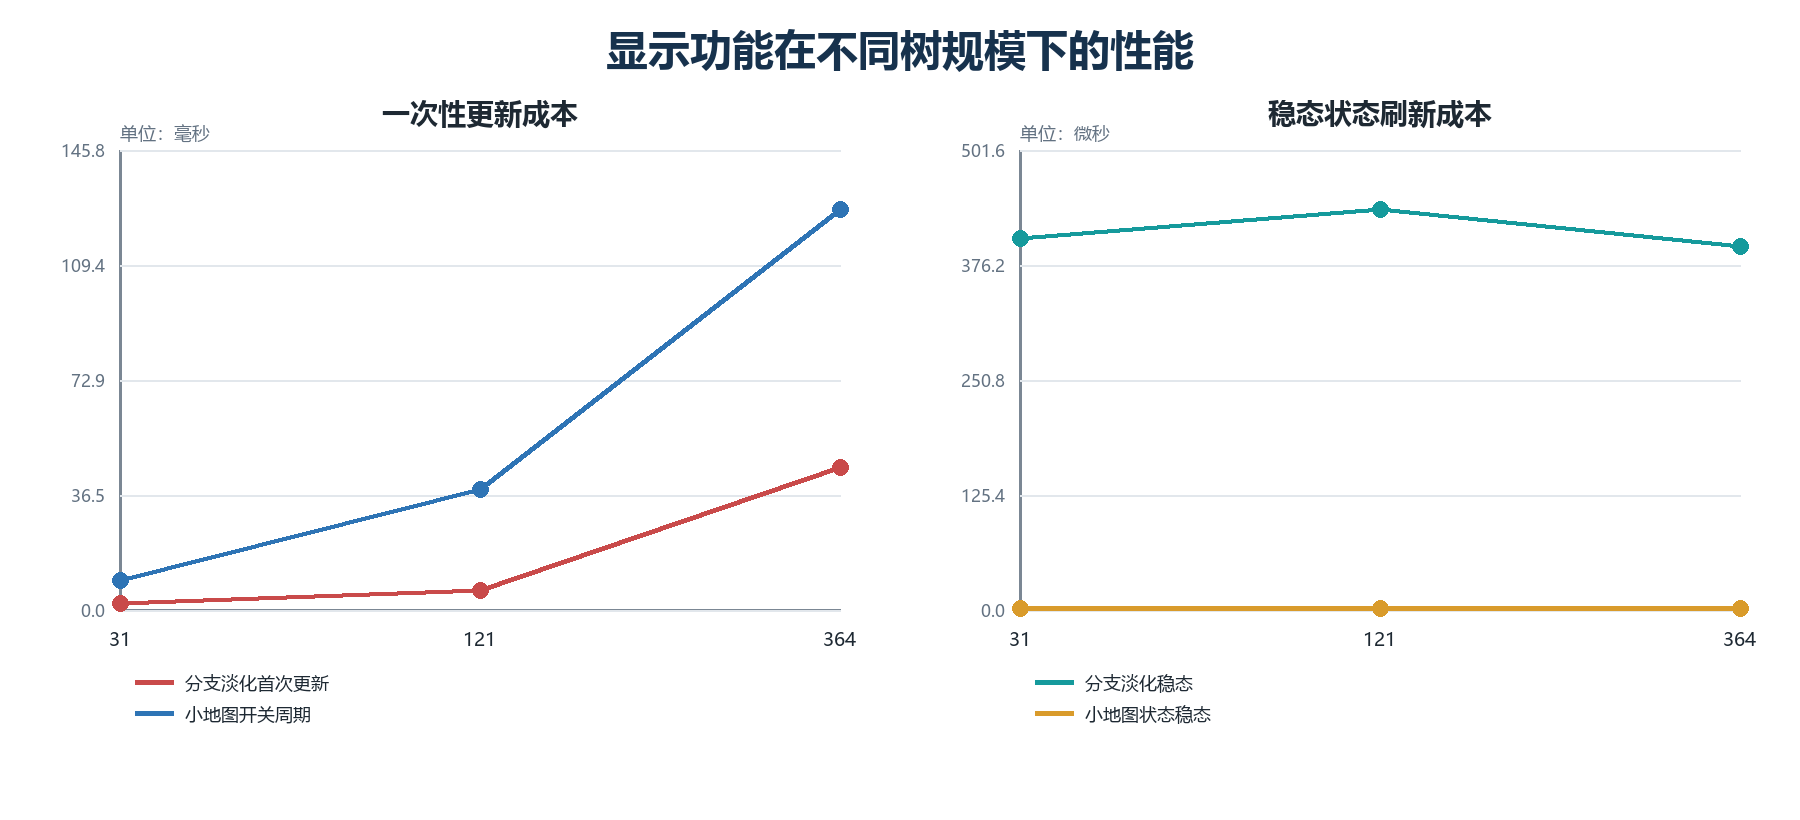
\includegraphics[width=0.9\textwidth]{figures/performance_scaling.png}
    \caption{Runtime tick scaling with the safe topology cache enabled and disabled.}
    \label{fig:performance}
\end{figure}

The data do not show a clear monotonic penalty from adding runners because the benchmark fixes total tick work approximately rather than running every actor for a fixed wall-clock duration. The valid interpretation is therefore within each size/load pair: cached and uncached conditions execute comparable work on the same machine. Cross-machine or production-frame claims require a different benchmark.

\section{Summary against research questions}

RQ1 is supported by the complete test matrix and complex game: the plugin authors, serialises, validates, executes and debugs non-trivial agent behaviour. RQ2 is answered at the instrumented-display level: compact, semantic, structural, salience and overview methods produced distinct measurable effects and passed real-renderer reset checks. Human readability remains unanswered. RQ3 is supported for the tested workload: exact-signature topology caching preserved semantics and substantially reduced median tick cost, especially on larger trees.
